\documentclass[11pt,a4paper]{article}
\usepackage[margin=22mm,top=21mm,bottom=22mm,headheight=15pt,headsep=9mm]{geometry}
\usepackage{fontspec}
\usepackage{amsmath}
\usepackage{unicode-math}
\defaultfontfeatures{Ligatures=TeX}
\setmainfont{Latin Modern Roman}
\setsansfont{Latin Modern Sans}
\setmonofont{Latin Modern Mono}
\setmathfont{Latin Modern Math}
\usepackage[table]{xcolor}
\definecolor{navy}{HTML}{203F53}
\definecolor{slate}{HTML}{526675}
\definecolor{paperblue}{HTML}{EDF2F5}
\usepackage{graphicx,booktabs,array,tabularx,caption,fancyhdr,pdflscape,titlesec,needspace}
\usepackage[unicode,colorlinks=true,linkcolor=navy,urlcolor=navy,citecolor=navy,bookmarksnumbered=true]{hyperref}
\hypersetup{pdftitle={US banking stress in March 2023},pdfauthor={Alessandro Capoccia},pdfsubject={Statistical detection, simulation validation and industry networks}}
\urlstyle{same}
\setlength{\parindent}{0pt}
\setlength{\parskip}{6pt}
\linespread{1.075}
\setlength{\emergencystretch}{1.5em}
\widowpenalty=10000\clubpenalty=10000
\pagestyle{fancy}\fancyhf{}
\fancyhead[L]{\sffamily\scriptsize\color{slate}ALESSANDRO CAPOCCIA}
\fancyhead[R]{\sffamily\scriptsize\color{slate}US BANKING STRESS | MARCH 2023}
\fancyfoot[L]{\sffamily\scriptsize\color{slate}Research report | 3 October 2026}
\fancyfoot[R]{\sffamily\small\color{navy}\thepage}
\renewcommand{\headrulewidth}{0pt}\renewcommand{\footrulewidth}{0pt}
\titleformat{\section}{\sffamily\Large\bfseries\color{navy}}{}{0pt}{}
\titleformat{\subsection}{\sffamily\normalsize\bfseries\color{navy}}{}{0pt}{}
\titlespacing*{\section}{0pt}{12pt}{9pt}
\titlespacing*{\subsection}{0pt}{10pt}{4pt}
\captionsetup{hypcap=false,font={small,sf},labelfont={bf,color=navy},textfont={color=slate},labelsep=period,skip=5pt,justification=raggedright,singlelinecheck=false}
\newcolumntype{L}[1]{>{\raggedright\arraybackslash}p{#1}}
\newcolumntype{C}[1]{>{\centering\arraybackslash}p{#1}}
\newcommand{\reporttablefont}{\fontsize{9.4}{11.7}\selectfont}
\begin{document}

{\sffamily\small\color{slate}EMPIRICAL FINANCE / METHODS AND EVIDENCE}\par\vspace{9pt}
{\sffamily\fontsize{28}{31}\selectfont\bfseries\color{navy}US banking stress\\in March 2023}\par\vspace{8pt}
{\sffamily\large\color{slate}Abnormal returns, statistical detection\\and industry networks}\par\vspace{10pt}
{\sffamily\normalsize Alessandro Capoccia\hfill 3 October 2026}\par\vspace{10pt}
\subsection*{Abstract}
This report examines daily US banking-industry returns during the March 2023 stress episode relative to a market model estimated in 2022. A daily threshold rule and a negative cumulative sum detector are calibrated to comparable probabilities of at least one alarm over an 81-observation Gaussian monitoring horizon. Simulations show that their relative performance depends on the form of the departure: CUSUM is more responsive to sustained negative mean shifts, whereas the threshold rule detects isolated negative shocks more often on the shock day. The nominal false-alarm budget does not transfer to the heavier-tail and empirical-residual baselines considered.

In the historical application, the threshold rule signals on 9 and 13 March, and CUSUM signals on 13 March. Banking cumulative abnormal return is $-$12.545 percentage points over 8\textendash{}31 March. Minimum spanning trees for 12 selected industries have lower total correlation distance in March, although banking's tree degree falls from three to one. Its average raw correlation peaks at 0.676 in March; the average becomes 0.052 after adjustment using fixed 2022 market exposures. That small adjusted average combines substantial positive and negative relationships. The evidence describes unusual performance and changes in estimated co-movement; it does not identify causal contagion or demonstrate crisis prediction.

\section*{1 Introduction}\addcontentsline{toc}{section}{1 Introduction}
The failures of Silicon Valley Bank and Signature Bank in March 2023 provide a setting in which to examine how statistical monitoring rules respond during financial stress. SVB announced balance-sheet restructuring on 8 March, experienced a large depositor run on 9 March and was closed on 10 March. Signature Bank closed on 12 March, when US authorities also announced depositor protection and additional bank funding \hyperlink{ref3}{[3]}, \hyperlink{ref4}{[4]}.

The analysis asks how unusual banking returns were relative to their prior market relationship, when two simple rules would flag negative abnormal performance, and how banking's position in a selected industry network differed across February, March and April. The unit of observation is an industry equity portfolio, rather than an individual bank or a deposit-flow series. All historical signals use completed daily returns. The project combines a retrospective case study with controlled simulations that make the detectors' behaviour and assumptions explicit.

\clearpage
\section*{2 Data and study design}\addcontentsline{toc}{section}{2 Data and study design}
The inputs are the Kenneth French 49 Industry Portfolios daily file and the Fama\textendash{}French daily research factors. The analysis selects the value-weighted industry-return section and retains the market excess return, Mkt-RF, and the risk-free return, RF \hyperlink{ref1}{[1]}, \hyperlink{ref2}{[2]}. Value weighting gives larger firms greater influence, so the results describe the portfolio's aggregate equity performance rather than the typical bank. Only the market factor is used; this is not a fitted three-factor model.

Industry portfolios are assigned using SIC industry classifications. The market factor represents a broad US equity portfolio less the risk-free return \hyperlink{ref1}{[1]}, \hyperlink{ref2}{[2]}. Source percentages are divided by 100 before calculation. Missing-value codes $-$99.99 and $-$999 are treated as missing. Dates are parsed explicitly and checked for ordering, duplicates and agreement between files. The retained 332 dates have no missing industry or selected factor values.

\begin{minipage}{\linewidth}\captionsetup{type=table}\caption{Estimation monitoring and descriptive windows}\reporttablefont\renewcommand{\arraystretch}{1.22}\begin{tabular}{@{}L{0.202857\dimexpr\linewidth-6\tabcolsep\relax}C{0.268571\dimexpr\linewidth-6\tabcolsep\relax}C{0.142857\dimexpr\linewidth-6\tabcolsep\relax}C{0.385714\dimexpr\linewidth-6\tabcolsep\relax}@{}}\toprule
{\sffamily\bfseries\color{navy}Window} & {\sffamily\bfseries\color{navy}Dates} & {\sffamily\bfseries\color{navy}Observations} & {\sffamily\bfseries\color{navy}Role}\\\midrule
Estimation & 3 Jan\textendash{}30 Dec 2022 & 251 & Fit the market benchmark\\
Monitoring & 3 Jan\textendash{}28 Apr 2023 & 81 & Apply frozen detectors\\
Pre-stress monitoring & 3 Jan\textendash{}7 Mar 2023 & 44 & Historical comparison\\
Stress & 8\textendash{}31 Mar 2023 & 18 & Historical comparison\\
After March & 3\textendash{}28 Apr 2023 & 19 & Historical comparison\\
Network windows & February / March / April 2023 & 19 / 23 / 19 & Monthly correlations and MSTs\\
\bottomrule\end{tabular}\end{minipage}\par\vspace{5pt}
Monitoring starts in January, before the event window, and retains any pre-event alarms. The March stress dates are a retrospective descriptive choice tied to the event timeline; they do not establish a known statistical change point. \textquotedblleft{}After March\textquotedblright{} is a calendar label, not a claim that banking stress ended in April. Network analysis uses the full calendar month of March, including 1\textendash{}7 March; its window differs from the 8\textendash{}31 March abnormal-performance summary.

\subsection*{Selected industry network}
The same 12 portfolio codes are used in all monthly networks: Banks, Insur, RlEst, Fin, Softw, Chips, Util, Oil, Mach, Trans, Rtail and Food. They cover banking and related financial categories together with technology, utilities, energy, machinery, transportation, retail and food. Codes are retained in tables and plots to make the calculations traceable to the source. Portfolio membership follows the source classification; labels such as Chips and Fin should not be read as a pure semiconductor portfolio or the entire financial sector. This selected subset is not a network of the entire economy, and its membership affects which MST edges are chosen.

\subsection*{Data vintage}
The supplied CSV headers identify the August 2026 CRSP database vintage. Historical values can therefore differ from those available to an analyst in March 2023. The exercise does not reconstruct an archived real-time information set. Original files and SHA-256 fingerprints are recorded in the project checkpoint; the report uses the same files as the verified notebook.

\clearpage
\section*{3 The market benchmark}\addcontentsline{toc}{section}{3 The market benchmark}
Let $r_{B,t}$ be the banking portfolio return on trading day t, $r_{M,t}$ the market return and $r_{f,t}$ the risk-free return. Define banking excess return $y_t$ = $r_{B,t}$ $-$ $r_{f,t}$ and market excess return $x_t$ = $r_{M,t}$ $-$ $r_{f,t}$. Mkt-RF already supplies $x_t$. The 2022 regression is

\begin{equation}y_t=\alpha+\beta x_t+\varepsilon_t\label{eq:model}\end{equation}
Here $\alpha$ is the intercept, $\beta$ is the slope measuring linear market sensitivity, and $\varepsilon_t$ is the deviation from the population linear specification. The market return is an observed regressor, not a variable determined within this model. A causal interpretation or an assumption of economic exogeneity is not required to construct the descriptive benchmark.

Ordinary least squares with an intercept is calculated directly from centred observations. With $\bar x$ and $\bar y$ denoting the 2022 sample means, the estimates are

\begin{equation}\hat\beta=\frac{\sum_t(x_t-\bar{x})(y_t-\bar{y})}{\sum_t(x_t-\bar{x})^2},\qquad\hat\alpha=\bar{y}-\hat\beta\bar{x}\label{eq:ols}\end{equation}
The in-sample residual is $e_t$ = $y_t$ $-$ $\widehat\alpha$ $-$ $\widehat\beta$$x_t$. Its estimated scale is $s_\varepsilon$ = $\sqrt{\sum_t e_t^2/(T-2)}$, where T = 251. The denominator accounts for the two fitted coefficients under the usual regression assumptions; it does not remove heteroskedasticity, dependence or parameter uncertainty.

\begin{minipage}{\linewidth}\captionsetup{type=table}\caption{Banking market model estimated in 2022}\reporttablefont\renewcommand{\arraystretch}{1.22}\begin{tabular}{@{}L{0.300000\dimexpr\linewidth-4\tabcolsep\relax}C{0.164286\dimexpr\linewidth-4\tabcolsep\relax}L{0.535714\dimexpr\linewidth-4\tabcolsep\relax}@{}}\toprule
{\sffamily\bfseries\color{navy}Quantity} & {\sffamily\bfseries\color{navy}Estimate} & {\sffamily\bfseries\color{navy}Interpretation}\\\midrule
Slope $\widehat\beta$ & 0.938687 & Market sensitivity in the estimation year\\
Daily intercept $\widehat\alpha$ & 0.00015945 & 0.015945 percentage points per day\\
Residual scale & 0.00850488 & 0.850488 percentage points per day\\
R squared & 0.756619 & Share of in-sample centred variation fitted\\
Residual lag-one correlation & 0.076929 & Descriptive serial-dependence check\\
Squared-residual lag-one correlation & 0.095006 & Descriptive volatility-dependence check\\
\bottomrule\end{tabular}\end{minipage}\par\vspace{5pt}
The model fits roughly 75.7\% of the centred variation in banking excess returns during 2022. A slope below one does not imply lower total banking volatility. The residual diagnostics do not establish independence, Gaussian tails or constant variance, and no significance claim is made for the intercept.

\subsection*{Abnormal returns in 2023}
\begin{equation}\mathrm{AR}_t=y_t-(\hat\alpha+\hat\beta x_t),\qquad z_t=\frac{\mathrm{AR}_t}{s_\varepsilon}\label{eq:abnormal}\end{equation}
$\mathrm{AR}_t$ is the deviation from the frozen 2022 benchmark; $z_t$ expresses it in units of the 2022 residual scale. Neither coefficients nor scale are re-estimated using March outcomes. \textquotedblleft{}Abnormal\textquotedblright{} is therefore model-relative and need not identify a bank-specific shock. Changes in market sensitivity or omitted common factors can also appear in $\mathrm{AR}_t$.

\clearpage
\section*{4 Detection rules and calibration}\addcontentsline{toc}{section}{4 Detection rules and calibration}
\subsection*{Daily threshold rule}
\begin{equation}\text{alarm at }t\quad\Longleftrightarrow\quad z_t\leq-c,\qquad c=3.22.\label{eq:threshold}\end{equation}
The threshold rule tests each observation separately. It responds immediately to sufficiently negative standardized abnormal returns, while moderate negative values do not accumulate across days. Positive returns are retained in the input series.

\subsection*{Negative CUSUM}
\begin{equation}\begin{aligned}\widetilde S_t&=\max\{0,S_{t-1}-z_t-k\},\qquad S_0=0,\quad k=0.5,\\ S_t&=\begin{cases}0,&\widetilde S_t\geq h\quad\text{(alarm)},\\\widetilde S_t,&\widetilde S_t<h,\end{cases}\qquad h=5.45.\end{aligned}\label{eq:cusum}\end{equation}
The provisional score $\widetilde S_t$ accumulates negative deviations after subtracting a reference allowance k. An alarm occurs when $\widetilde S_t$ $\geq$ h, with h = 5.45. Following an alarm, the state used on the next day is reset to zero; otherwise $S_t$ = $\widetilde S_t$. Figures show the provisional score before this reset, so the boundary crossing remains visible.

A value $z_t$ < $-$0.5 raises the score; a value above $-$0.5 lowers it, subject to the zero floor. Positive observations therefore counteract accumulated evidence. This lower-sided recursion follows the tabular CUSUM approach \hyperlink{ref5}{[5]}. For independent $N(0,1)$ observations versus a negative mean shift of size $\delta$, the log-likelihood-ratio increment is $\delta$($-$$z_t$$-$$\delta$/2). Setting k = $\delta$/2 gives k = 0.5 for a one-standard-deviation reference shift. This is a design interpretation under a Gaussian model, not an assumption that financial returns actually follow that distribution.

\subsection*{Comparable simulated alarm budgets}
The calibration target is approximately a 5\% probability of at least one alarm in 81 observations of independent $N(0,1)$ noise. The monitoring horizon matches January\textendash{}April 2023. It is not a 5\% probability per day or a 5\% probability that a historical alarm is false. CUSUM uses the same reset rule in calibration, scenario simulations and the historical application.

\begin{minipage}{\linewidth}\captionsetup{type=table}\caption{Final Gaussian calibration with 100000 replicates}\reporttablefont\renewcommand{\arraystretch}{1.22}\begin{tabular}{@{}L{0.221429\dimexpr\linewidth-4\tabcolsep\relax}C{0.364286\dimexpr\linewidth-4\tabcolsep\relax}C{0.414286\dimexpr\linewidth-4\tabcolsep\relax}@{}}\toprule
{\sffamily\bfseries\color{navy}Detector} & {\sffamily\bfseries\color{navy}Fixed setting} & {\sffamily\bfseries\color{navy}Probability of any alarm}\\\midrule
Threshold & c = 3.22 & 5.077\%\\
CUSUM & k = 0.5 and h = 5.45 & 5.086\%\\
\bottomrule\end{tabular}\end{minipage}\par\vspace{5pt}
These results use seed 123. Near a probability of 0.05, the Monte Carlo standard error with 100,000 replicates is approximately 0.00069, or 0.069 percentage points. Parameters and seeds were examined during calibration, so this run is not described as an untouched holdout. The final settings remain fixed in every subsequent comparison. They were not retuned to produce particular March alarm dates.

Calibration provides a controlled basis for comparing the rules. Its external relevance depends on whether the simulated noise resembles the observations being monitored. The next section evaluates that dependence directly.

\clearpage
\section*{5 Sensitivity to the noise distribution}\addcontentsline{toc}{section}{5 Sensitivity to the noise distribution}
The first sensitivity checks introduce no deliberate change within a simulated monitoring path. They retain the same detector settings and measure the probability of at least one alarm over 81 observations. The non-Gaussian experiments each use 10,000 replicates.

\begin{minipage}{\linewidth}\captionsetup{type=table}\caption{Alarm probabilities under alternative baseline constructions}\reporttablefont\renewcommand{\arraystretch}{1.22}\begin{tabular}{@{}L{0.657143\dimexpr\linewidth-4\tabcolsep\relax}C{0.171429\dimexpr\linewidth-4\tabcolsep\relax}C{0.171429\dimexpr\linewidth-4\tabcolsep\relax}@{}}\toprule
{\sffamily\bfseries\color{navy}Baseline} & {\sffamily\bfseries\color{navy}Threshold} & {\sffamily\bfseries\color{navy}CUSUM}\\\midrule
Independent $N(0,1)$ & 5.077\% & 5.086\%\\
Independent standardized t with 5 degrees of freedom & 29.51\% & 9.15\%\\
2022 residual bootstrap with block length 1 & 47.24\% & 7.00\%\\
2022 residual bootstrap with block length 5 & 41.86\% & 24.68\%\\
\bottomrule\end{tabular}\end{minipage}\par\vspace{5pt}
\subsection*{Heavy tails}
Student t draws with five degrees of freedom are multiplied by $\sqrt{3/5}$, giving variance one. The larger alarm rates therefore reflect a distributional change beyond a simple increase in variance. Five degrees of freedom is an illustrative choice rather than a fitted estimate. The threshold rule is particularly sensitive to this heavier lower tail.

\subsection*{Empirical residual resampling}
The empirical pool contains the 251 standardized banking residuals from 2022. With block length one, draws are independent resamples from that finite pool. With block length five, overlapping candidate five-day blocks are sampled with replacement, concatenated and trimmed to 81 observations. This retains ordering within each selected block. The seed is 2028 for both block lengths.

Exactly two pool observations satisfy z $\leq$ $-$3.22. Conditional on this empirical pool, independent resampling gives the following exact probability of at least one threshold alarm:

\begin{equation}1-\left(1-\frac{2}{251}\right)^{81}=0.476911\label{eq:tail_probability}\end{equation}
The simulated 0.4724 is consistent with that calculation. The threshold rate is already high without preserving time order because the empirical lower tail contains extreme observations. The increase in CUSUM alarms from 7.00\% to 24.68\% when five-day blocks are used is consistent with sensitivity to local runs. Ordinary moving blocks also weight boundary observations differently, so the comparison does not isolate serial dependence perfectly.

These experiments show why a Gaussian 5\% calibration cannot be attached mechanically to historical signals. Resampling does not solve uncertainty about the baseline: 2022 may itself contain changing conditions, and its estimated extreme lower tail depends on only two observations. The procedure cannot generate extremes absent from the pool. With the regression residual scale used here, the pool's empirical variance is 249/251 rather than exactly one.

\clearpage
\section*{6 Detection under controlled changes}\addcontentsline{toc}{section}{6 Detection under controlled changes}
Each scenario uses 1,000 independent Gaussian paths of 81 observations. A change is inserted at zero-based index 40, the 41st observation. For sustained changes, 41 observations remain, including the change day. Monitoring continues after any earlier false alarm under the reset policy. Detection probability counts a post-change alarm, and delay is measured from the change index to the first such alarm. Mean delay is reported only among detected paths, so it must be read alongside detection probability. These are unconditional post-change alarm probabilities under continued monitoring, rather than probabilities conditional on no earlier alarm.

\begin{minipage}{\linewidth}\centering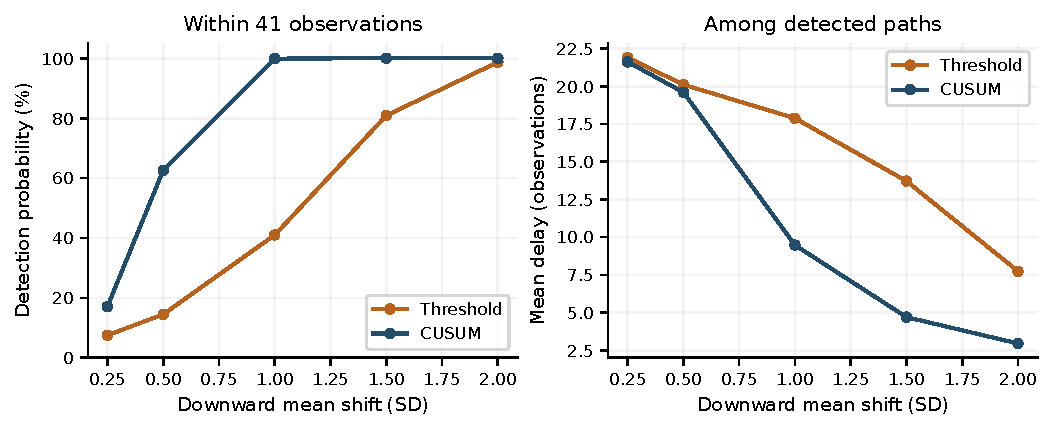
\includegraphics[width=\linewidth]{figures/shift_simulation.pdf}\captionof{figure}{Persistent negative mean shifts. Shift size is measured in baseline standard deviations. Each point uses 1,000 replicates; seed 2026 is reset for each scenario. The delay panel excludes missed detections, and the detected subsets differ between rules.}\end{minipage}\par\vspace{4pt}
\begin{minipage}{\linewidth}\captionsetup{type=table}\caption{Representative change scenarios}\reporttablefont\renewcommand{\arraystretch}{1.22}\begin{tabular}{@{}L{0.657143\dimexpr\linewidth-4\tabcolsep\relax}C{0.171429\dimexpr\linewidth-4\tabcolsep\relax}C{0.171429\dimexpr\linewidth-4\tabcolsep\relax}@{}}\toprule
{\sffamily\bfseries\color{navy}Scenario and metric} & {\sffamily\bfseries\color{navy}Threshold} & {\sffamily\bfseries\color{navy}CUSUM}\\\midrule
Persistent shift of 1 SD: detection probability & 41.0\% & 99.9\%\\
Persistent shift of 1 SD: mean delay if detected & 17.88 & 9.47\\
Single shock of 3 SD: alarm on the shock day & 41.8\% & 4.1\%\\
Volatility multiplier 2: post-change alarm probability & 87.7\% & 73.2\%\\
Volatility multiplier 2: mean delay if detected & 12.51 & 16.21\\
\bottomrule\end{tabular}\end{minipage}\par\vspace{5pt}
CUSUM has higher post-change detection probabilities for the sustained negative mean shifts tested here. A daily threshold is more responsive to isolated negative shocks on the shock day. These metrics use different evaluation horizons; a same-day shock hit rate cannot be compared directly with a 41-observation detection probability as if they measured the same outcome. With 1,000 replicates, the binomial Monte Carlo standard error is at most 1.58 percentage points. Small numerical differences should therefore not be treated as precise rankings.

In the volatility experiment, observations from the change point onward are multiplied by a positive factor while their distribution remains centred at zero. At a multiplier of two, variance quadruples. Both detectors alarm frequently despite the absence of an imposed negative mean shift. An alarm therefore indicates a departure relative to the calibrated baseline but does not identify its cause. Full parameter grids are provided in the appendix.

\clearpage
\section*{7 Historical alarm dates}\addcontentsline{toc}{section}{7 Historical alarm dates}
The frozen rules are applied to all 81 monitoring observations. The threshold rule alarms on 9 and 13 March; CUSUM alarms on 13 March only. Neither produces another alarm in the January\textendash{}April sample. These signals become available after the corresponding daily return is observed.

\begin{minipage}{\linewidth}\captionsetup{type=table}\caption{Event context and computed signals}\reporttablefont\renewcommand{\arraystretch}{1.22}\begin{tabular}{@{}L{0.150000\dimexpr\linewidth-4\tabcolsep\relax}C{0.607143\dimexpr\linewidth-4\tabcolsep\relax}C{0.242857\dimexpr\linewidth-4\tabcolsep\relax}@{}}\toprule
{\sffamily\bfseries\color{navy}Date in 2023} & {\sffamily\bfseries\color{navy}Event context} & {\sffamily\bfseries\color{navy}Computed signal}\\\midrule
8 March & SVB restructuring and planned capital raise \hyperlink{ref3}{[3]} & Neither rule\\
9 March & SVB depositor run \hyperlink{ref3}{[3]} & Threshold\\
10 March & SVB closure and FDIC receivership \hyperlink{ref3}{[3]} & Neither rule\\
12 March & Signature closure and depositor measures \hyperlink{ref4}{[4]} & Sunday without a daily return\\
13 March & First trading session after weekend measures & Threshold and CUSUM\\
\bottomrule\end{tabular}\end{minipage}\par\vspace{5pt}
\begin{minipage}{\linewidth}\centering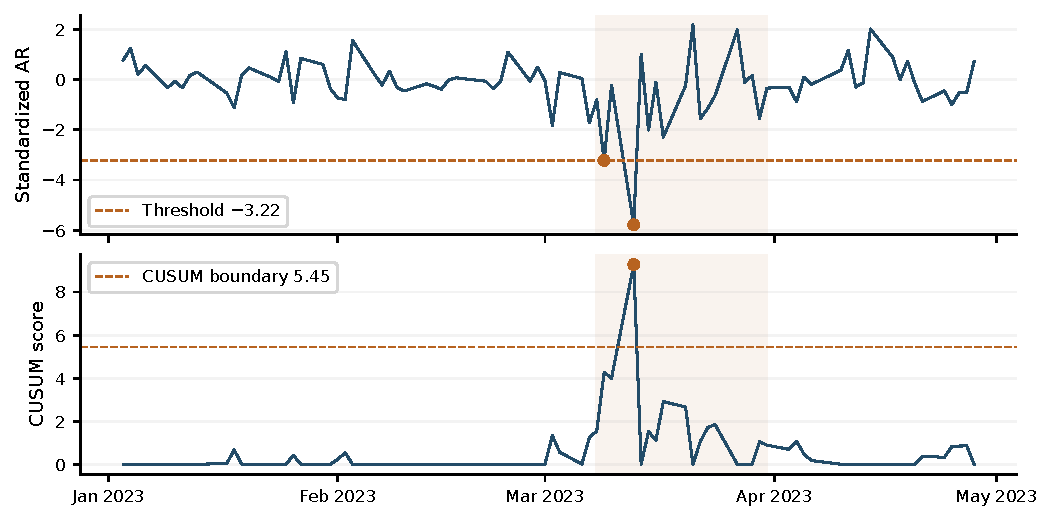
\includegraphics[width=\linewidth]{figures/historical_detectors.pdf}\captionof{figure}{Standardized banking abnormal returns and CUSUM scores before reset. Shading marks 8\textendash{}31 March. Markers identify computed alarm dates. Both series use the 2022 benchmark and fixed detector parameters.}\end{minipage}\par\vspace{4pt}
On 9 March, z = $-$3.221442 only narrowly crosses the $-$3.22 threshold. This signal is sensitive to small changes in the cutoff or input values. On 13 March, z = $-$5.781141 is more extreme and the provisional CUSUM score reaches 9.283481. From a zero state, that day alone would contribute 5.281141, below h = 5.45; earlier accumulation matters.

The 9 March signal occurs during unfolding stress, not before the relevant news. The two-trading-observation gap between detector alarm dates is not a detection delay from a known historical change point. The 13 March return reflects a session following several developments; the analysis does not attribute it to one announcement or identify an intervention effect.

\clearpage
\section*{8 Historical abnormal performance}\addcontentsline{toc}{section}{8 Historical abnormal performance}
\begin{minipage}{\linewidth}\captionsetup{type=table}\caption{Banking abnormal returns by descriptive window}\reporttablefont\renewcommand{\arraystretch}{1.22}\begin{tabular}{@{}L{0.250000\dimexpr\linewidth-8\tabcolsep\relax}C{0.078571\dimexpr\linewidth-8\tabcolsep\relax}C{0.207143\dimexpr\linewidth-8\tabcolsep\relax}C{0.200000\dimexpr\linewidth-8\tabcolsep\relax}C{0.264286\dimexpr\linewidth-8\tabcolsep\relax}@{}}\toprule
{\sffamily\bfseries\color{navy}Window} & {\sffamily\bfseries\color{navy}Days} & {\sffamily\bfseries\color{navy}Mean AR\newline pp per day} & {\sffamily\bfseries\color{navy}CAR\newline pp} & {\sffamily\bfseries\color{navy}AR standard\newline deviation pp}\\\midrule
3 Jan\textendash{}7 Mar & 44 & $-$0.016 & $-$0.709 & 0.582\\
8\textendash{}31 Mar & 18 & $-$0.697 & $-$12.545 & 1.573\\
3\textendash{}28 Apr & 19 & 0.028 & 0.529 & 0.661\\
\bottomrule\end{tabular}\end{minipage}\par\vspace{5pt}
Here pp denotes percentage points. Cumulative abnormal return (CAR) is the sum of arithmetic daily abnormal returns. It is not a compounded portfolio return or an identified causal loss. Window lengths differ, which matters when comparing totals. Within-window standard deviations use the sample divisor n$-$1.

\begin{minipage}{\linewidth}\centering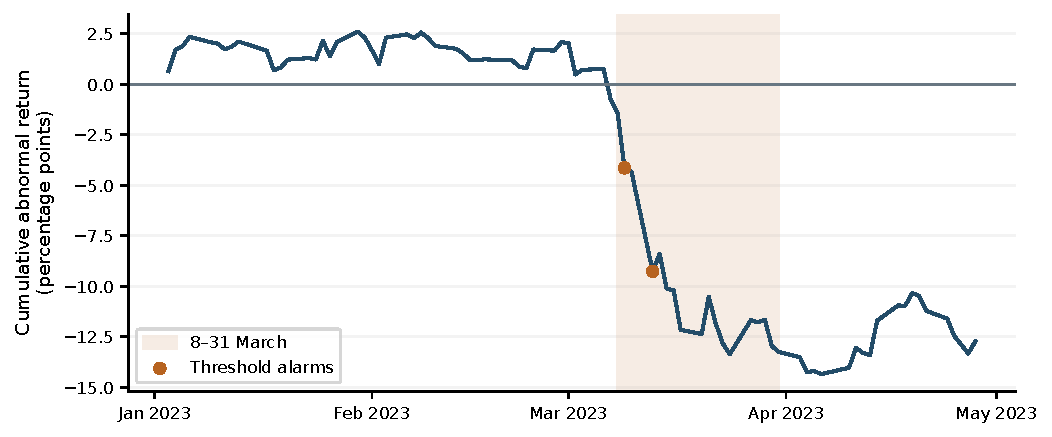
\includegraphics[width=\linewidth]{figures/car.pdf}\captionof{figure}{Cumulative banking abnormal return from January 2023. The line sums deviations from the frozen 2022 market benchmark; orange markers show threshold alarm dates. Its endpoint is $-$12.725 percentage points.}\end{minipage}\par\vspace{4pt}
Stress-window abnormal-return variability is about 2.7 times that of the pre-stress monitoring window. The decline is partly concentrated in two extreme observations. The 9 and 13 March abnormal returns sum to $-$7.657 percentage points, approximately 61\% of the net stress-window CAR. This proportion uses a net total and is not a variance contribution.

The remaining 16 stress-window days still sum to $-$4.888 percentage points, with a mean of $-$0.306 percentage points per day. Fourteen of all 18 stress days have negative abnormal returns, and the median is $-$0.415 percentage points. The exclusion of the two alarm dates is a post hoc descriptive check, selected after viewing the results. It supports a combination of concentrated extreme days and broader negative abnormal performance without establishing a permanent mean shift.

April's slightly positive average abnormal return does not reverse the earlier shortfall. Likewise, the absence of additional alarms does not imply the absence of further underperformance: later negative returns can remain individually below the threshold magnitude or fail to accumulate enough CUSUM evidence.

\clearpage
\section*{9 Industry networks and sampling sensitivity}\addcontentsline{toc}{section}{9 Industry networks and sampling sensitivity}
Monthly Pearson correlation $\widehat\rho_{ij}$ measures linear co-movement between raw industry returns and is sensitive to extreme observations. The correlation distance used in financial-network analysis \hyperlink{ref6}{[6]} is

\begin{equation}d_{ij}=\sqrt{2(1-\hat\rho_{ij})}\label{eq:distance}\end{equation}
The complete graph has 12 industries and 66 undirected edges. An MST selects 11 edges connecting all industries at minimum total distance. The custom Kruskal algorithm sorts edges and uses Union-Find with path compression and union by component size to reject cycles; sorting dominates its $O(E\log E)$ complexity. Higher positive correlation gives a shorter edge; perfect negative correlation gives distance two.

Every tree has 11 edges, one connected component and a total weight matching SciPy within numerical tolerance \hyperlink{ref7}{[7]}. SciPy also uses Kruskal: this checks the custom implementation, not the financial meaning of its distances.

\begin{minipage}{\linewidth}\captionsetup{type=table}\caption{Observed trees and banking correlations}\reporttablefont\renewcommand{\arraystretch}{1.22}\begin{tabular}{@{}L{0.214286\dimexpr\linewidth-6\tabcolsep\relax}C{0.257143\dimexpr\linewidth-6\tabcolsep\relax}C{0.185714\dimexpr\linewidth-6\tabcolsep\relax}C{0.342857\dimexpr\linewidth-6\tabcolsep\relax}@{}}\toprule
{\sffamily\bfseries\color{navy}Month} & {\sffamily\bfseries\color{navy}MST total\newline distance} & {\sffamily\bfseries\color{navy}Banks\newline degree} & {\sffamily\bfseries\color{navy}Banks mean raw\newline correlation}\\\midrule
February & 7.698 & 3 & 0.547\\
March & 6.159 & 1 & 0.676\\
April & 7.721 & 1 & 0.522\\
\bottomrule\end{tabular}\end{minipage}\par\vspace{5pt}
March's tree is shorter. Banking's mean equally weights 11 correlations, excluding itself. It rises while degree falls because the MST depends on competing edges. Banking's neighbours are Fin, Chips and Mach in February, then only Fin. Overlap is 5/11 for February\textendash{}March and 4/11 for each other pair. Its median moves from 0.718 to 0.711, so co-movement did not strengthen uniformly.

\subsection*{Bootstrap edge selection}
Each of 1,000 within-month bootstrap samples resamples whole daily rows, recomputes correlations and constructs a new MST. Joint observations are preserved, but serial ordering is lost. Seed 2026 is set once before the February\textendash{}March\textendash{}April loop.

\begin{minipage}{\linewidth}\captionsetup{type=table}\caption{Stability of edges in the observed trees}\reporttablefont\renewcommand{\arraystretch}{1.22}\begin{tabular}{@{}L{0.214286\dimexpr\linewidth-6\tabcolsep\relax}C{0.257143\dimexpr\linewidth-6\tabcolsep\relax}C{0.342857\dimexpr\linewidth-6\tabcolsep\relax}C{0.185714\dimexpr\linewidth-6\tabcolsep\relax}@{}}\toprule
{\sffamily\bfseries\color{navy}Month} & {\sffamily\bfseries\color{navy}Banks\textendash{}Fin\newline frequency} & {\sffamily\bfseries\color{navy}Mean original-edge\newline frequency} & {\sffamily\bfseries\color{navy}Edges at\newline least 70\%}\\\midrule
February & 94.6\% & 62.4\% & 3\\
March & 78.3\% & 68.0\% & 7\\
April & 89.9\% & 67.4\% & 6\\
\bottomrule\end{tabular}\end{minipage}\par\vspace{5pt}
Mean frequency is the average fraction of original edges retained; 70\% is a descriptive cutoff. March's larger sample also affects comparisons. Frequencies establish neither persistent links nor significant distance changes. Banks\textendash{}Insur is absent from March's tree but appears in 40.3\% of bootstrap trees: frequent Banks\textendash{}Fin selection does not establish stable banking degree.

\clearpage\newgeometry{left=16mm,right=16mm,top=16mm,bottom=16mm}\begin{landscape}\thispagestyle{empty}\setlength{\parskip}{2pt}\captionsetup{font={footnotesize,sf}}
\section*{10 Monthly correlation and tree comparisons}\addcontentsline{toc}{section}{10 Monthly correlation and tree comparisons}
\begin{minipage}{\linewidth}\centering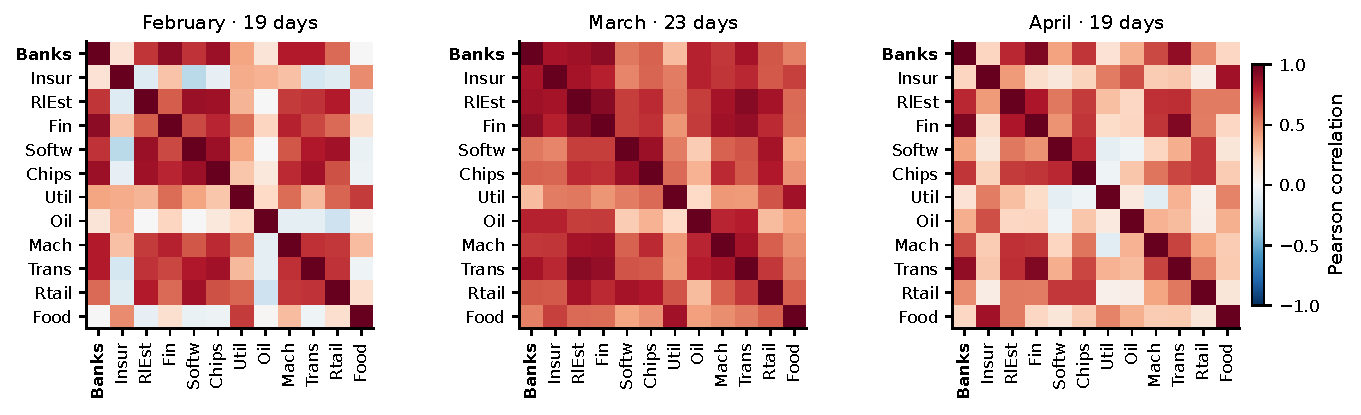
\includegraphics[width=.82\linewidth]{figures/heatmaps.pdf}\captionof{figure}{Raw-return correlations, with a common industry order and colour scale. March shows broader positive co-movement, while some pairs weaken. Calculations use the supplied French industry returns.}\end{minipage}\par\vspace{4pt}
\begin{minipage}{\linewidth}\centering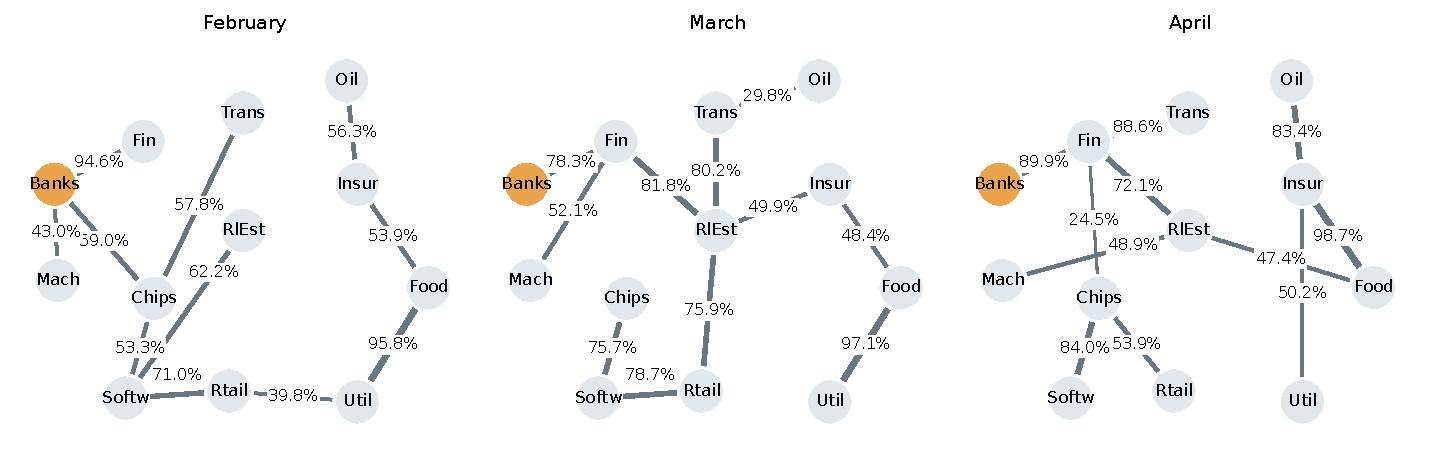
\includegraphics[width=.82\linewidth]{figures/mst.pdf}\captionof{figure}{Monthly MSTs and bootstrap edge frequencies (one decimal place). Banks is orange; thicker edges are selected more often. Fixed node positions aid comparison; drawn lengths have no economic meaning, and crossings are not nodes.}\end{minipage}\par\vspace{4pt}
\vfill{\sffamily\scriptsize\color{slate}Alessandro Capoccia | US banking stress 2023\hfill\thepage}\end{landscape}\restoregeometry\setlength{\parskip}{6pt}\captionsetup{font={small,sf}}
\section*{11 Correlations after benchmark adjustment}\addcontentsline{toc}{section}{11 Correlations after benchmark adjustment}
A separate 2022 market model is estimated for each industry using the same excess-return \mbox{OLS} calculation as for Banks. The coefficients remain fixed when computing February\textendash{}April 2023 abnormal returns:

\begin{equation}\mathrm{AR}_{i,t}=(r_{i,t}-r_{f,t})-[\hat\alpha_i+\hat\beta_i(r_{M,t}-r_{f,t})]\label{eq:adjustment}\end{equation}
Here i identifies the industry. Correlations use the adjusted series; Banks reproduces the historical abnormal returns. Appendix B lists the frozen coefficients. A fixed intercept does not affect correlation, whereas the time-varying market adjustment does. Adjusted MSTs and their bootstrap are outside this analysis.

\begin{minipage}{\linewidth}\captionsetup{type=table}\caption{Banking correlations before and after benchmark adjustment}\reporttablefont\renewcommand{\arraystretch}{1.22}\begin{tabular}{@{}L{0.171429\dimexpr\linewidth-8\tabcolsep\relax}C{0.228571\dimexpr\linewidth-8\tabcolsep\relax}C{0.257143\dimexpr\linewidth-8\tabcolsep\relax}C{0.171429\dimexpr\linewidth-8\tabcolsep\relax}C{0.171429\dimexpr\linewidth-8\tabcolsep\relax}@{}}\toprule
{\sffamily\bfseries\color{navy}Month} & {\sffamily\bfseries\color{navy}Banks mean\newline raw correlation} & {\sffamily\bfseries\color{navy}Banks mean\newline adjusted correlation} & {\sffamily\bfseries\color{navy}Banks\textendash{}Fin\newline raw} & {\sffamily\bfseries\color{navy}Banks\textendash{}Fin\newline adjusted}\\\midrule
February & 0.547 & 0.026 & 0.895 & 0.746\\
March & 0.676 & 0.052 & 0.894 & 0.711\\
April & 0.522 & 0.081 & 0.930 & 0.807\\
\bottomrule\end{tabular}\end{minipage}\par\vspace{5pt}
The March peak in the raw average disappears after adjustment. However, the adjusted average is close to zero because positive and negative values offset each other. The pairwise estimates reveal that heterogeneity. Banks\textendash{}Fin remains strongly positive in every month after adjustment (0.746, 0.711 and 0.807), showing that the small overall average conceals a strong pairwise association.

\begin{minipage}{\linewidth}\captionsetup{type=table}\caption{Correlation between banking and other industries after adjustment}\reporttablefont\renewcommand{\arraystretch}{1.22}\begin{tabular}{@{}L{0.314286\dimexpr\linewidth-6\tabcolsep\relax}C{0.228571\dimexpr\linewidth-6\tabcolsep\relax}C{0.228571\dimexpr\linewidth-6\tabcolsep\relax}C{0.228571\dimexpr\linewidth-6\tabcolsep\relax}@{}}\toprule
{\sffamily\bfseries\color{navy}Industry} & {\sffamily\bfseries\color{navy}February} & {\sffamily\bfseries\color{navy}March} & {\sffamily\bfseries\color{navy}April}\\\midrule
Fin & 0.746 & 0.711 & 0.807\\
Oil & 0.202 & 0.602 & 0.122\\
Insur & 0.402 & 0.568 & $-$0.252\\
RlEst & $-$0.282 & 0.465 & 0.326\\
Trans & 0.068 & 0.299 & 0.685\\
Mach & 0.282 & 0.084 & 0.380\\
Food & 0.046 & $-$0.041 & $-$0.284\\
Util & $-$0.200 & $-$0.300 & $-$0.119\\
Rtail & $-$0.580 & $-$0.567 & $-$0.294\\
Softw & $-$0.535 & $-$0.604 & $-$0.423\\
Chips & 0.136 & $-$0.640 & $-$0.055\\
\bottomrule\end{tabular}\end{minipage}\par\vspace{5pt}
Oil, Insur and RlEst retain positive March associations after adjustment, whereas Food's raw March increase is absent. Banks\textendash{}Chips changes from +0.591 in raw March returns to $-$0.640 after adjustment. Comparing months instead, its adjusted correlation changes from +0.136 in February to $-$0.640 in March. These are distinct comparisons.

This removes the component predicted by 2022 exposures. Changed exposures and omitted factors can remain. Correlation reductions are not variance decompositions. Negative adjusted correlation means opposite deviations around monthly means, not necessarily opposite signs of daily raw or abnormal returns.

\clearpage
\section*{12 Limitations and conclusion}\addcontentsline{toc}{section}{12 Limitations and conclusion}
\subsection*{Interpretive limits}
The findings are conditional on a simple benchmark, selected windows and a finite sample. A single estimation year may not represent a stable reference distribution. The in-sample residual diagnostics are descriptive, and the historical scale and coefficients are estimated. Most simulations condition on a known standardized baseline rather than propagating that estimation uncertainty. Alternative false-alarm budgets and parameter-uncertainty sensitivity were not evaluated.

The heavier-tail and empirical-residual experiments show that a common Gaussian alarm budget does not carry over to other distributions. The historical signals consequently have no generic 5\% significance interpretation. Detection probabilities and conditional delays are separate outcomes: methods can detect different subsets of paths, and earlier simulated false alarms do not exclude a path from subsequent monitoring.

Monthly correlation estimates use only 19\textendash{}23 observations. An unstable period may combine different conditions within a single month. Ordinary row bootstrap reweights the observed days, cannot introduce missing shocks and does not preserve temporal dependence. A block bootstrap could retain local ordering but would not solve changing regimes or the limited sample size. No network block bootstrap, matched-length comparison or formal test of between-month tree-weight differences was performed.

An MST compresses 66 pairwise relationships to 11 selected edges and always connects every included node. A missing edge need not imply a weak correlation, and banking's degree is only one feature of its position in the selected tree. The network is neither a balance-sheet exposure map nor a directed transmission model. Industry selection, common shocks and estimation noise can alter the tree without causal contagion.

The benchmark adjustment is also limited. Coefficients fixed at their 2022 values need not remove the market component prevailing in 2023. Small mean adjusted correlations can hide strong relationships of opposite signs. Historical estimates use a later data vintage, and all daily alarms require the day's return. Neither the event study nor the network comparison establishes prediction or the causal effect of an announcement.

\subsection*{Conclusion}
Banking experienced substantial negative abnormal performance during March 2023 relative to its 2022 market relationship. The threshold and CUSUM signals identify different features of that performance, consistent with their simulated responses to isolated and sustained departures. The noise-distribution experiments show that calibration assumptions are material to interpreting any alarm.

The selected raw-return network has a lower MST distance in March, while banking's tree degree declines and its average raw correlation rises. Those observations are compatible because they describe different network properties. Adjustment using 2022 market exposures removes the March peak in average banking correlation but leaves positive and negative pairwise associations. Taken together, the results support a descriptive account of unusual banking performance and heterogeneous industry co-movement, with explicit limits on inference.

\clearpage
\setcounter{table}{0}\renewcommand{\thetable}{A\arabic{table}}
\section*{Appendix A  Simulation grids and run settings}\addcontentsline{toc}{section}{Appendix A  Simulation grids and run settings}
\begin{minipage}{\linewidth}\captionsetup{type=table}\caption{Persistent negative mean shifts with 1000 replicates per setting}\reporttablefont\renewcommand{\arraystretch}{1.22}\begin{tabular}{@{}L{0.092857\dimexpr\linewidth-8\tabcolsep\relax}C{0.235714\dimexpr\linewidth-8\tabcolsep\relax}C{0.214286\dimexpr\linewidth-8\tabcolsep\relax}C{0.235714\dimexpr\linewidth-8\tabcolsep\relax}C{0.221429\dimexpr\linewidth-8\tabcolsep\relax}@{}}\toprule
{\sffamily\bfseries\color{navy}Shift\newline SD} & {\sffamily\bfseries\color{navy}Threshold\newline detection \%} & {\sffamily\bfseries\color{navy}CUSUM\newline detection \%} & {\sffamily\bfseries\color{navy}Threshold\newline mean delay} & {\sffamily\bfseries\color{navy}CUSUM\newline mean delay}\\\midrule
0.25 & 7.5 & 17.1 & 21.89 & 21.61\\
0.50 & 14.5 & 62.6 & 20.10 & 19.60\\
1.00 & 41.0 & 99.9 & 17.88 & 9.47\\
1.50 & 80.9 & 100.0 & 13.71 & 4.70\\
2.00 & 98.7 & 100.0 & 7.74 & 2.95\\
\bottomrule\end{tabular}\end{minipage}\par\vspace{5pt}
Delay is measured in observations, with zero denoting an alarm on the change day. It excludes paths without a post-change alarm. A 100\% observed simulation rate is not a guarantee for future samples. Changes start at index 40 and remain through index 80.

\begin{minipage}{\linewidth}\captionsetup{type=table}\caption{Single negative shocks with 1000 replicates per setting}\reporttablefont\renewcommand{\arraystretch}{1.22}\begin{tabular}{@{}L{0.200000\dimexpr\linewidth-4\tabcolsep\relax}C{0.400000\dimexpr\linewidth-4\tabcolsep\relax}C{0.400000\dimexpr\linewidth-4\tabcolsep\relax}@{}}\toprule
{\sffamily\bfseries\color{navy}Shock size SD} & {\sffamily\bfseries\color{navy}Threshold same-day hit \%} & {\sffamily\bfseries\color{navy}CUSUM same-day hit \%}\\\midrule
0 & 0.0 & 0.2\\
1 & 1.5 & 0.3\\
2 & 11.4 & 2.0\\
3 & 41.8 & 4.1\\
4 & 80.0 & 13.2\\
5 & 96.6 & 32.8\\
\bottomrule\end{tabular}\end{minipage}\par\vspace{5pt}
The isolated shock is inserted only at index 40. Size zero is a designated-day false-alarm control, not an 81-day false-alarm rate.

\begin{minipage}{\linewidth}\captionsetup{type=table}\caption{Volatility multipliers with 1000 replicates per setting}\reporttablefont\renewcommand{\arraystretch}{1.22}\begin{tabular}{@{}L{0.128571\dimexpr\linewidth-8\tabcolsep\relax}C{0.214286\dimexpr\linewidth-8\tabcolsep\relax}C{0.200000\dimexpr\linewidth-8\tabcolsep\relax}C{0.228571\dimexpr\linewidth-8\tabcolsep\relax}C{0.228571\dimexpr\linewidth-8\tabcolsep\relax}@{}}\toprule
{\sffamily\bfseries\color{navy}Multiplier} & {\sffamily\bfseries\color{navy}Threshold\newline detection \%} & {\sffamily\bfseries\color{navy}CUSUM\newline detection \%} & {\sffamily\bfseries\color{navy}Threshold\newline mean delay} & {\sffamily\bfseries\color{navy}CUSUM\newline mean delay}\\\midrule
1.00 & 3.6 & 2.6 & 22.94 & 18.96\\
1.25 & 19.3 & 13.3 & 20.03 & 19.80\\
1.50 & 47.2 & 35.7 & 17.36 & 19.13\\
2.00 & 87.7 & 73.2 & 12.51 & 16.21\\
\bottomrule\end{tabular}\end{minipage}\par\vspace{5pt}
A multiplier of one inserts no change; its entries describe alarms in the post-index-40 observation window. Larger multipliers change variance by the square of the multiplier while preserving the simulated mean. Settings and standardization remain fixed.

\subsection*{Randomness and replication}
Random seeds are 123 for Gaussian calibration, 2027 for the t baseline, and 2028 for residual bootstrap, reset for each block length. Change scenarios reset seed 2026 for each setting. The MST bootstrap sets seed 2026 once before the February\textendash{}March\textendash{}April loop. Replicate counts are reported with each experiment.

\clearpage
\setcounter{table}{0}\renewcommand{\thetable}{B\arabic{table}}
\section*{Appendix B  Industry coefficients and reproducibility}\addcontentsline{toc}{section}{Appendix B  Industry coefficients and reproducibility}
The following coefficients use excess returns expressed as decimals and the 251 trading observations in 2022. Alpha is a daily intercept, not an annualized return. All coefficients remain fixed when constructing the 2023 adjusted series.

\begin{minipage}{\linewidth}\captionsetup{type=table}\caption{Frozen 2022 market-model coefficients}\reporttablefont\renewcommand{\arraystretch}{1.22}\begin{tabular}{@{}L{0.400000\dimexpr\linewidth-4\tabcolsep\relax}C{0.300000\dimexpr\linewidth-4\tabcolsep\relax}C{0.300000\dimexpr\linewidth-4\tabcolsep\relax}@{}}\toprule
{\sffamily\bfseries\color{navy}Industry code} & {\sffamily\bfseries\color{navy}Daily alpha} & {\sffamily\bfseries\color{navy}Beta}\\\midrule
Banks & 0.00015945 & 0.938687\\
Insur & 0.00082797 & 0.608952\\
RlEst & -0.00040717 & 1.185749\\
Fin & 0.00030764 & 1.036942\\
Softw & -0.00056645 & 1.318042\\
Chips & -0.00005637 & 1.349151\\
Util & 0.00056578 & 0.517986\\
Oil & 0.00272849 & 0.633670\\
Mach & 0.00044376 & 1.037270\\
Trans & -0.00012820 & 0.965709\\
Rtail & -0.00035916 & 1.116706\\
Food & 0.00060988 & 0.402854\\
\bottomrule\end{tabular}\end{minipage}\par\vspace{5pt}
\subsection*{Files and execution}
The companion analysis\_reviewed.ipynb contains data parsing, \mbox{OLS} calculations, the custom threshold and CUSUM rules, Union-Find and Kruskal implementations, simulations and network outputs. Its 102 code cells were executed in source order in a fresh Python process during review. A successful local VS Code notebook run was subsequently confirmed by the author.

Place 49\_Industry\_Portfolios\_Daily.csv and F-F\_Research\_Data\_Factors\_daily.csv in data/raw beneath the project directory, as expected by the notebook, and run all cells in order. These are the supplied files with vintage 202608; a fresh download may contain revised observations. The notebook is the computational source of truth. Plots in this report use the same analytical inputs, with publication formatting.

The verification environment used Python 3.12.14, NumPy 2.3.5, pandas 2.2.3, Matplotlib 3.10.8 and SciPy 1.17.0. The local user environment reported Python 3.14.4. These versions document the reviewed execution; they are not a claim that both environments are identical.

\subsection*{Scope of verification}
Checks covered alarm dates, historical summaries, all simulation grids, bootstrap frequencies, all 12 coefficient pairs and adjusted correlations. Each monthly tree has 11 edges, one connected component and a total weight matching SciPy. Adjusted Banks returns reproduce the original banking abnormal-return series. These checks establish computational agreement for the supplied data, not validity of the statistical assumptions.

\clearpage
\section*{References}\addcontentsline{toc}{section}{References}
Sources provide data definitions, historical context and methodological background. All reported estimates and simulations are calculations from the supplied data. The source pages were consulted during preparation and review in October 2026.

\hypertarget{ref1}{}\needspace{3\baselineskip}{\small\textbf{[1] Kenneth R French Data Library.} 49 Industry Portfolios and portfolio construction. Daily value-weighted returns are taken from the supplied CSV.\par{\footnotesize\url{https://mba.tuck.dartmouth.edu/pages/faculty/ken.french/Data_Library/det_49_ind_port.html}}}\par\vspace{3pt}
\hypertarget{ref2}{}\needspace{3\baselineskip}{\small\textbf{[2] Kenneth R French Data Library.} Description of Fama/French Factors. Definitions of Mkt-RF and RF.\par{\footnotesize\url{https://mba.tuck.dartmouth.edu/pages/faculty/ken.french/Data_Library/f-f_factors.html}}}\par\vspace{3pt}
\hypertarget{ref3}{}\needspace{3\baselineskip}{\small\textbf{[3] Board of Governors of the Federal Reserve System.} Evolution of Silicon Valley Bank. Review of supervision and regulation, April 2023; updated 18 May 2023.\par{\footnotesize\url{https://www.federalreserve.gov/publications/2023-April-SVB-Evolution-of-Silicon-Valley-Bank.htm}}}\par\vspace{3pt}
\hypertarget{ref4}{}\needspace{3\baselineskip}{\small\textbf{[4] US Treasury Federal Reserve and FDIC.} Joint Statement, 12 March 2023, 6:15 p.m. EDT.\par{\footnotesize\url{https://www.federalreserve.gov/newsevents/pressreleases/monetary20230312b.htm}}}\par\vspace{3pt}
\hypertarget{ref5}{}\needspace{3\baselineskip}{\small\textbf{[5] NIST and SEMATECH.} e-Handbook of Statistical Methods, section 6.3.2.3, CUSUM Control Charts.\par{\footnotesize\url{https://www.itl.nist.gov/div898/handbook/pmc/section3/pmc323.htm}}}\par\vspace{3pt}
\hypertarget{ref6}{}\needspace{3\baselineskip}{\small\textbf{[6] Rosario N Mantegna.} Hierarchical Structure in Financial Markets. Preprint cond-mat/9802256, 1998.\par{\footnotesize\url{https://arxiv.org/abs/cond-mat/9802256}}}\par\vspace{3pt}
\hypertarget{ref7}{}\needspace{3\baselineskip}{\small\textbf{[7] SciPy documentation.} scipy.sparse.csgraph.minimum\_spanning\_tree. Reference implementation and graph conventions.\par{\footnotesize\url{https://docs.scipy.org/doc/scipy/reference/generated/scipy.sparse.csgraph.minimum_spanning_tree.html}}}\par\vspace{3pt}
\subsection*{Source-file fingerprints}
SHA-256 fingerprints identify the precise CSVs used. Upload suffixes such as (2) are not part of the filenames expected by the notebook.

{\footnotesize\texttt{49\_Industry\_Portfolios\_Daily.csv}\par\texttt{63cc949d0335ff5416e598b0e10a0ef4}\texttt{d2a3d9afa7360433d9b5dafd50326499}}\par
{\footnotesize\texttt{F-F\_Research\_Data\_Factors\_daily.csv}\par\texttt{c2dc30c9e89eeea05a689c81fb426f4d}\texttt{76711270733b3731997615cbdff5b247}}\par
\end{document}